\documentclass[12pt, a4paper]{article} %determina o tamanho da fonte, o tipo de papel e o tipo de documento.

\setlength{\parindent}{1.0 cm} %tamanho do espaço para começar o parágrafo.
\setlength{\parskip}{0.5cm} %tamanho do espaço entre os parágrafos.

%Aqui ficam os pacotes utilizados para formatação do documento de modo geral:

\usepackage[utf8]{inputenc} 
\usepackage{indentfirst} %Coloca espaços nos inícios de parágrafos automaticamente. 
\usepackage[brazilian]{babel} %
\usepackage{amsmath}
\usepackage[hmargin=3cm, vmargin=2.5cm, bmargin=2.5cm]{geometry}
\usepackage{multicol}
\usepackage{graphicx} %para poder inserir imagens
\usepackage{subfig}
\usepackage{booktabs} 
\usepackage{hyperref} %para poder adicionar links e hiperlinks
\usepackage{float} %para poder posicionar as imagens


\usepackage{listings} %para poder incluir códigos
\usepackage{xcolor}
\definecolor{codegreen}{rgb}{0,0.6,0}
\definecolor{codegray}{rgb}{0.5,0.5,0.5}
\definecolor{codepurple}{rgb}{0.58,0,0.82}
\definecolor{backcolour}{rgb}{0.95,0.95,0.92}
\lstdefinestyle{mystyle}{
    backgroundcolor=\color{backcolour},   
    commentstyle=\color{codegreen},
    keywordstyle=\color{magenta},
    numberstyle=\tiny\color{codegray},
    stringstyle=\color{codepurple},
    basicstyle=\ttfamily\footnotesize,
    breakatwhitespace=false,         
    breaklines=true,                 
    captionpos=b,                    
    keepspaces=true,                 
    numbers=left,                    
    numbersep=5pt,                  
    showspaces=false,                
    showstringspaces=false,
    showtabs=false,                  
    tabsize=2,
    morecomment={l}[!],
    language=[77]Fortran,
}
\lstset{style=mystyle}

\begin{document} %começa alguma coisa,neste caso, o documento, sempre importante lembrar de colocar o \end{} para não dar erro 
	
	\begin{titlepage}
		\begin{center}
\Huge{Universidade de São Paulo}\\
\large{Instituto de Física de São Carlos}\\
\vspace{20pt}
\vspace{200pt}
\textbf{Lista 3}\\
\vspace{8cm}
		\end{center}

\begin{flushleft}
\begin{tabbing}
Pedro Calligaris Delbem 5255417\\
\end{tabbing}
\vspace{0.5cm}
Professor: Attilio Cucchieri\\		
		\end{flushleft}
	
		\begin{center}
			\vspace{\fill}
	Abril de 2025	
		\end{center}
	\end{titlepage}

%####################################################################### SUMÁRIO
	\tableofcontents 
	\thispagestyle{empty}
	\newpage
%#########################################################################

\section{The Numerov Algorithm}

    \subsection{Exerc\'icio 1}

        Tarefa: Reolver a equa\c{c}\~ao de Poisson para $\hat{\phi}(r)$ definido por $\frac{\hat{\phi}(r)}{r} := \phi(r)$ onde $\phi(r)$ \'e o potencial eletrost\'atico e a densidade de carga \'e $\rho(r) = \frac{e^{-r}}{8 \pi}$, considerando simetria esf\'erica.
        
        Deve-se resolver das seguintes maneiras:
        \begin{itemize} 
            \item Pelo algoritmo de Numerov
            \begin{itemize}
                \item Escolhendo $\hat{\phi}(0)$ e $\hat{\phi}(\delta r)$, para $r \approx 0$
                \item Escolhendo $\hat{\phi}(0)$ e $\hat{\phi}(\delta r)$, r muito grande (o equivalente num\'erico a $r \to \infty$)
            \end{itemize}
            \item Analiticamente
        \end{itemize}

        Primeiro deve-se manipular a equa\c{c}\~ao de Poisson de modo a obter uma equa\c{c}\~ao para $\hat{\phi}(r)$

        A equa\c{c}\~ao de Poisson \'e:
        \begin{equation*}
            \nabla^{2} \phi(r) = -4\pi \rho(r)
        \end{equation*}

        Sabemos que $\nabla^{2}$ em coordenadas esf\'ericas \'e:
        \begin{equation*}
            \nabla^{2} = \frac{1}{r^{2}} \left( \frac{\partial}{\partial r} \left( r^{2} \frac{\partial}{\partial r} \right) + \frac{1}{\sin \theta}\frac{\partial}{\partial \theta} \left( \sin \theta \frac{\partial}{\partial \theta} \right) + \frac{1}{r \sin^{2} \theta} \frac{\partial^{2}}{\partial \phi^{2}} \right)
        \end{equation*}

        Pela simetria radial reduzimos  para:

        \begin{equation*}
            \nabla^{2} = \frac{1}{r^{2}} \frac{\partial}{\partial r} \left( r^{2} \frac{\partial}{\partial r} \right)
        \end{equation*}

        Substituimos $\frac{\hat{\phi}(r)}{r} := \phi(r)$:

        \begin{equation*}
            \nabla^{2} \phi(r) = \frac{1}{r^{2}} \frac{\partial}{\partial r} \left( r^{2} \frac{\partial}{\partial r} \left( \frac{\hat{\phi}(r)}{r} \right) \right)
        \end{equation*}

        Aplicando as derivadas:

        \begin{equation*}
            \nabla^{2} \phi(r) = \frac{1}{r}\frac{\partial^{2}}{\partial r^{2}} \hat{\phi}(r)
        \end{equation*}

        Substituindo na equa\c{c}\~ao de Poisson:

        \begin{equation*}
            \frac{1}{r} \frac{d^{2} \hat{\phi}(r)}{dr^{2}} = -4\pi \rho(r) = -\frac{e^{-r}}{2}
        \end{equation*}

        Assim, obtemos:

        \begin{equation*}
            \frac{d^{2} \hat{\phi}(r)}{dr^{2}} = -\frac{re^{-r}}{2}
        \end{equation*}

        As escolhas para $\hat{\phi}(r)$ para r $\approx$ 0 e $r \to \infty$ s\~ao arbitr\'arias, e portanto toma-se $\hat{\phi}(0)$ = -1 e $\hat{\phi}(\infty)$ = 0, baseando-se nos fatos - primeiro de que a segunda derivada \'e negativa e segundo de que a densidade de carga tende a zero quando r tende ao infinito.
        J\'a para o primeiro passo do algoritmo de Numerov crescente, temos que expandir $\hat{\phi}(r)$ em torno de r = 0:
        \begin{equation*}
            \hat{\phi}(r) = \hat{\phi}(0) + \hat{\phi}'(0)r + O(r^{2})
        \end{equation*}
        Mas como $\hat{\phi}(0)$ = -1, e para r $\approx$ 0, $\hat{\phi}'(0) = -4\pi \rho(0)\delta r$ = -$\frac{\delta r}{2}$, temos que:
        \begin{equation*}
            \hat{\phi}(r) = -1 - \frac{r}{2} + O(r^{2})
        \end{equation*}
        Assim, para o primeiro passo do algoritmo de Numerov, temos que:
        \begin{equation*}
            \hat{\phi}(\delta r) = -1 - \frac{\delta r}{2}
        \end{equation*}
        E para o algoritmo decrescente, temos que expandir em torno de r muito grande (=: R) o que pela mesma l\'ogica nos dar\'a:
        \begin{equation*}
            \hat{\phi}(R - \delta r) = 0
        \end{equation*}
        Uma vez que $\hat{\phi}'(R - \delta r)$ = $-4\pi \rho(R - \delta r)\delta r \approx$  0.

        \subsubsection{Resolu\c{c}\~ao Anal\'itica}

            Integrando a equa\c{c}\~ao, com rela\c{c}\~ao ao r duas vezes, obtemos:

            \begin{equation*}
                \hat{\phi}(r) = e^{-r}\left(1 + \frac{r}{2}\right) + C_{1}r + C_{2}
            \end{equation*}

            As escolhas para $\hat{\phi}(r)$ para r $\approx$ 0 e $r \to \infty$ s\~ao arbitr\'arias, mas devem ser escolhidas em conson\^ancia com as escolhas para as solu\c{c}\~oes num\'ericas. Assim, toma-se $\hat{\phi}(0)$ = -1 e $\hat{\phi}(\infty)$ = 0 e obtemos:

            \begin{equation*}
                C_{1} = 0 \quad \text{e} \quad C_{2} = 0
            \end{equation*}
            
            E deste modo a solu\c{c}\~ao anal\'itica \'e:

            \begin{equation*}
                \hat{\phi}(r) = e^{-r}\left(1 + \frac{r}{2}\right)
            \end{equation*}

        Resultados:

        Compilou-se o código com:

            gfortran P1-5255417-ex-1.f90 -Wall -Wextra -pedantic -o P1-5255417-ex-1.exe

        Plotando os resultados obtidos pelos algoritmos de Numerov crescente, decrescente e pela solu\c{c}\~ao anal\'itica, obtemos os seguintes resultados - para v\'arios valores de $\delta r$:
        \begin{figure}[H]
            \centering
            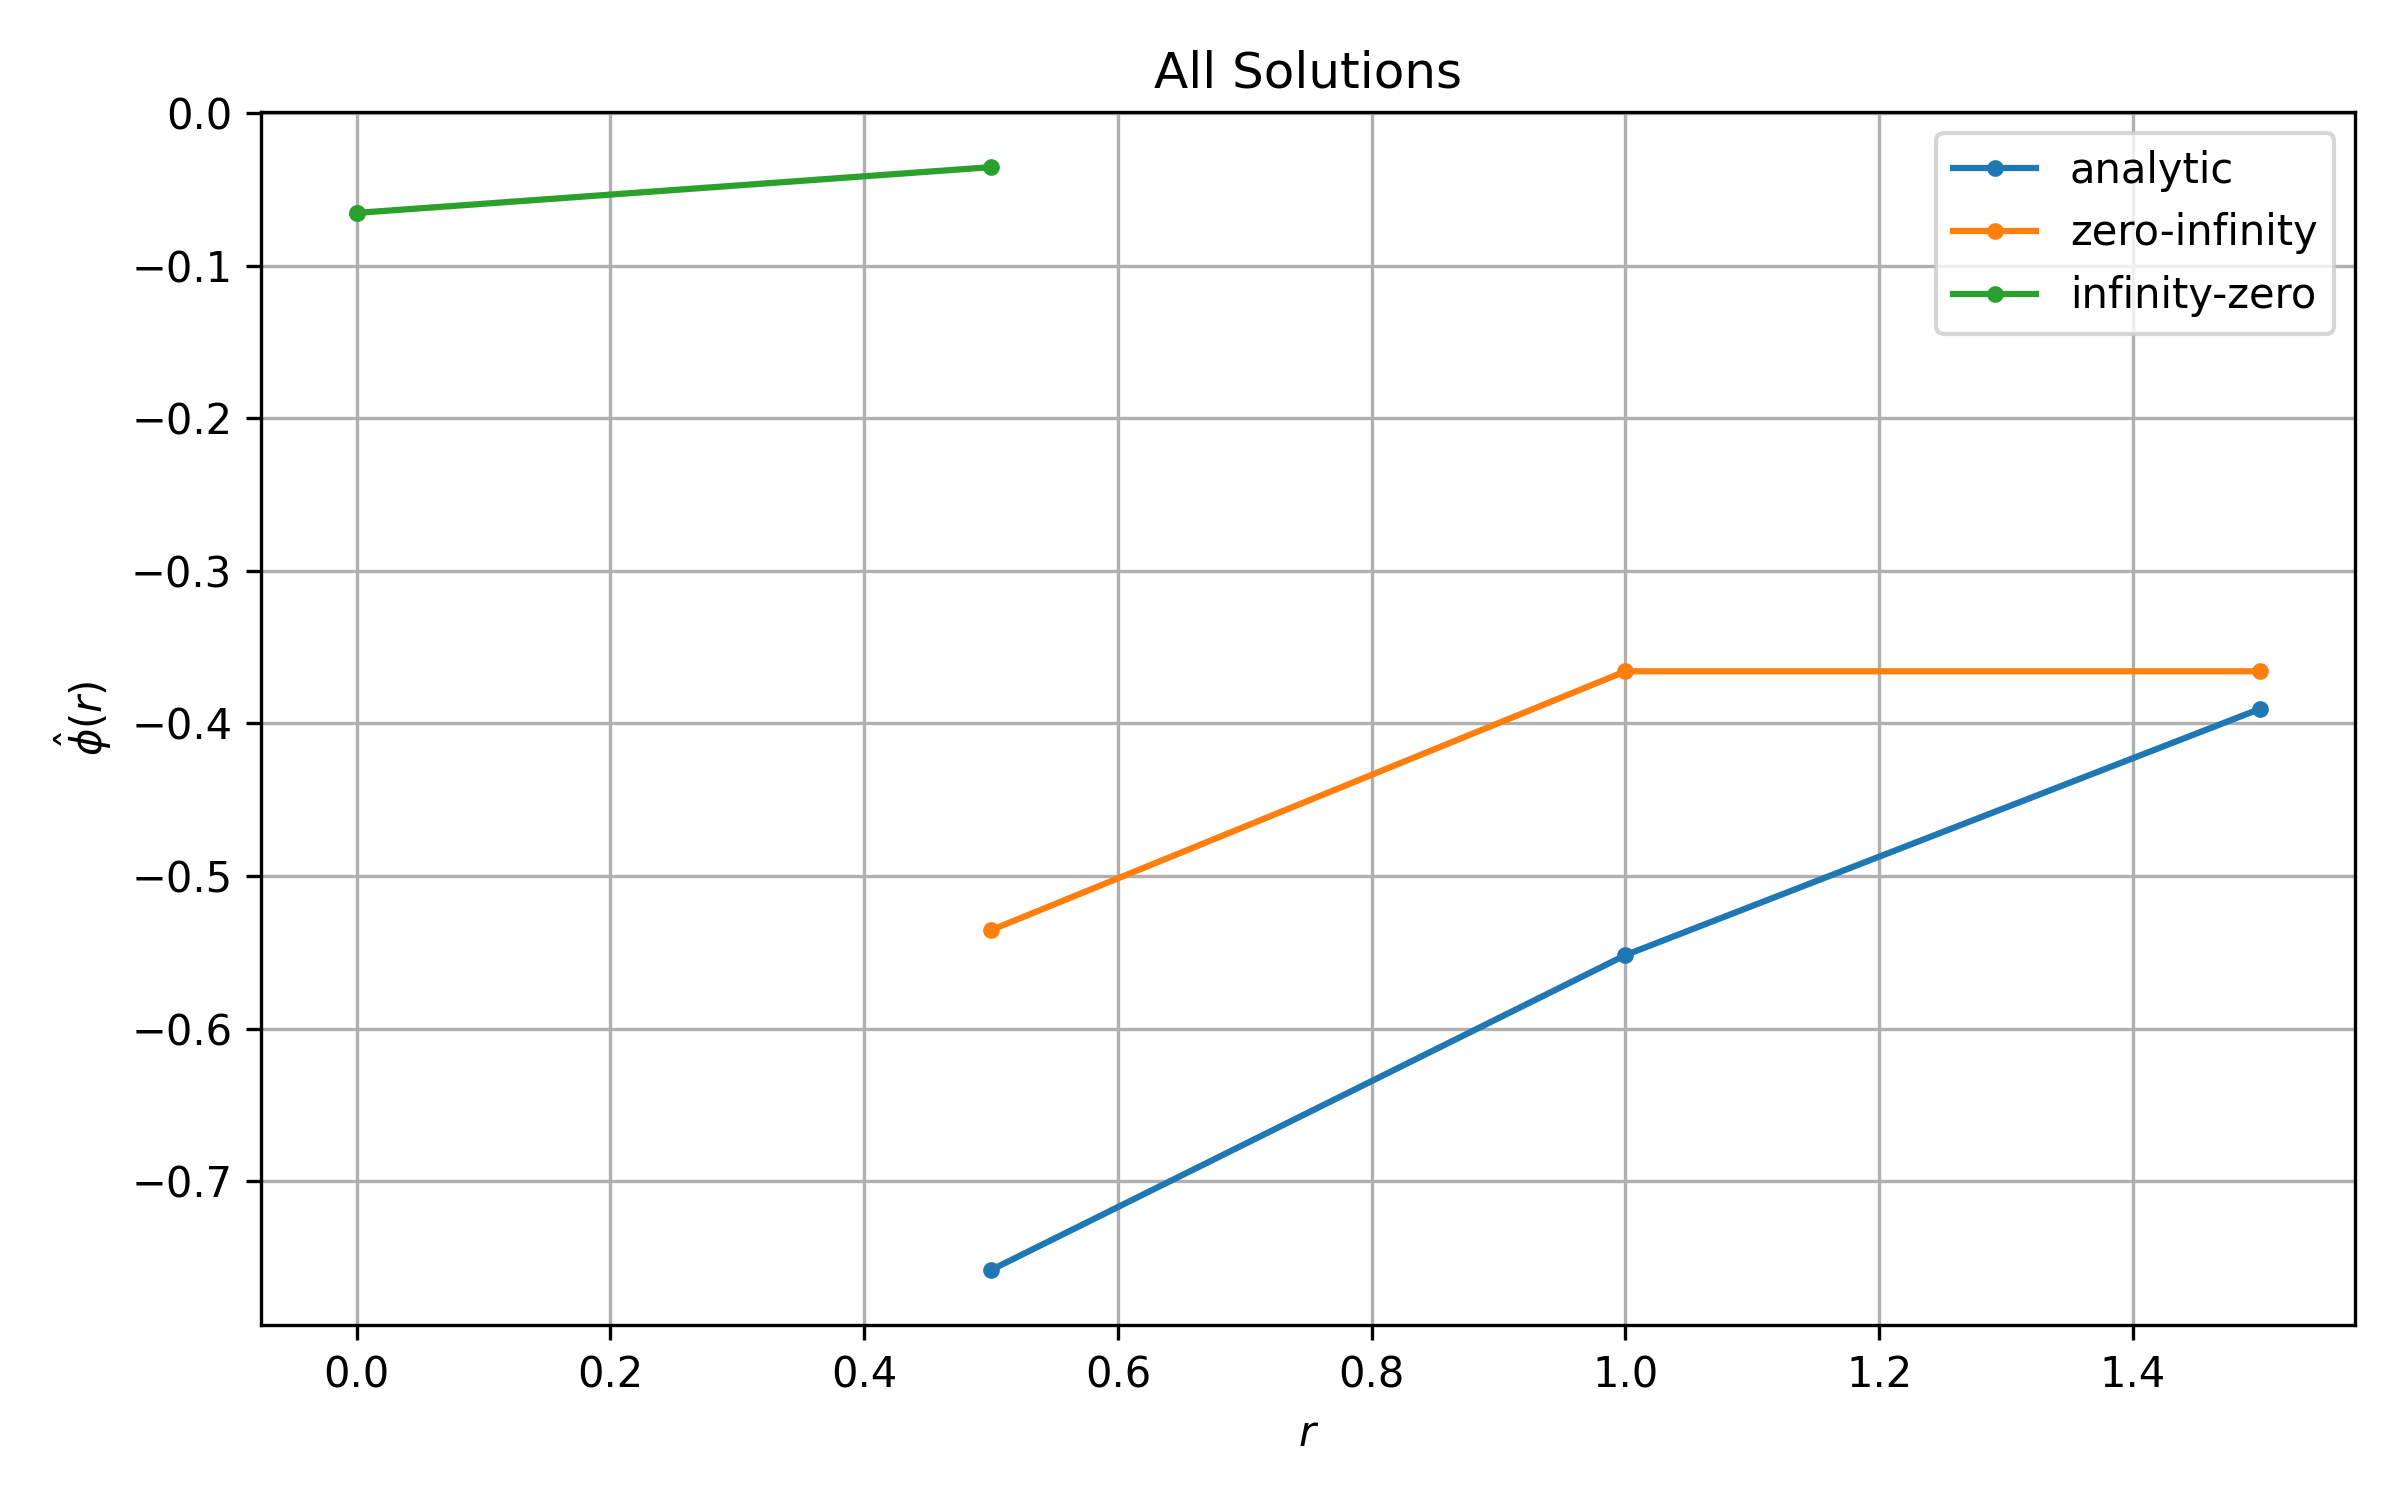
\includegraphics[scale=0.7]{../images/all-plots-0.5.png}
            \caption{Resultados para $\delta r = 0.5$}
            \label{fig:all-plots-0.5}
        \end{figure}
        \begin{figure}[H]
            \centering
            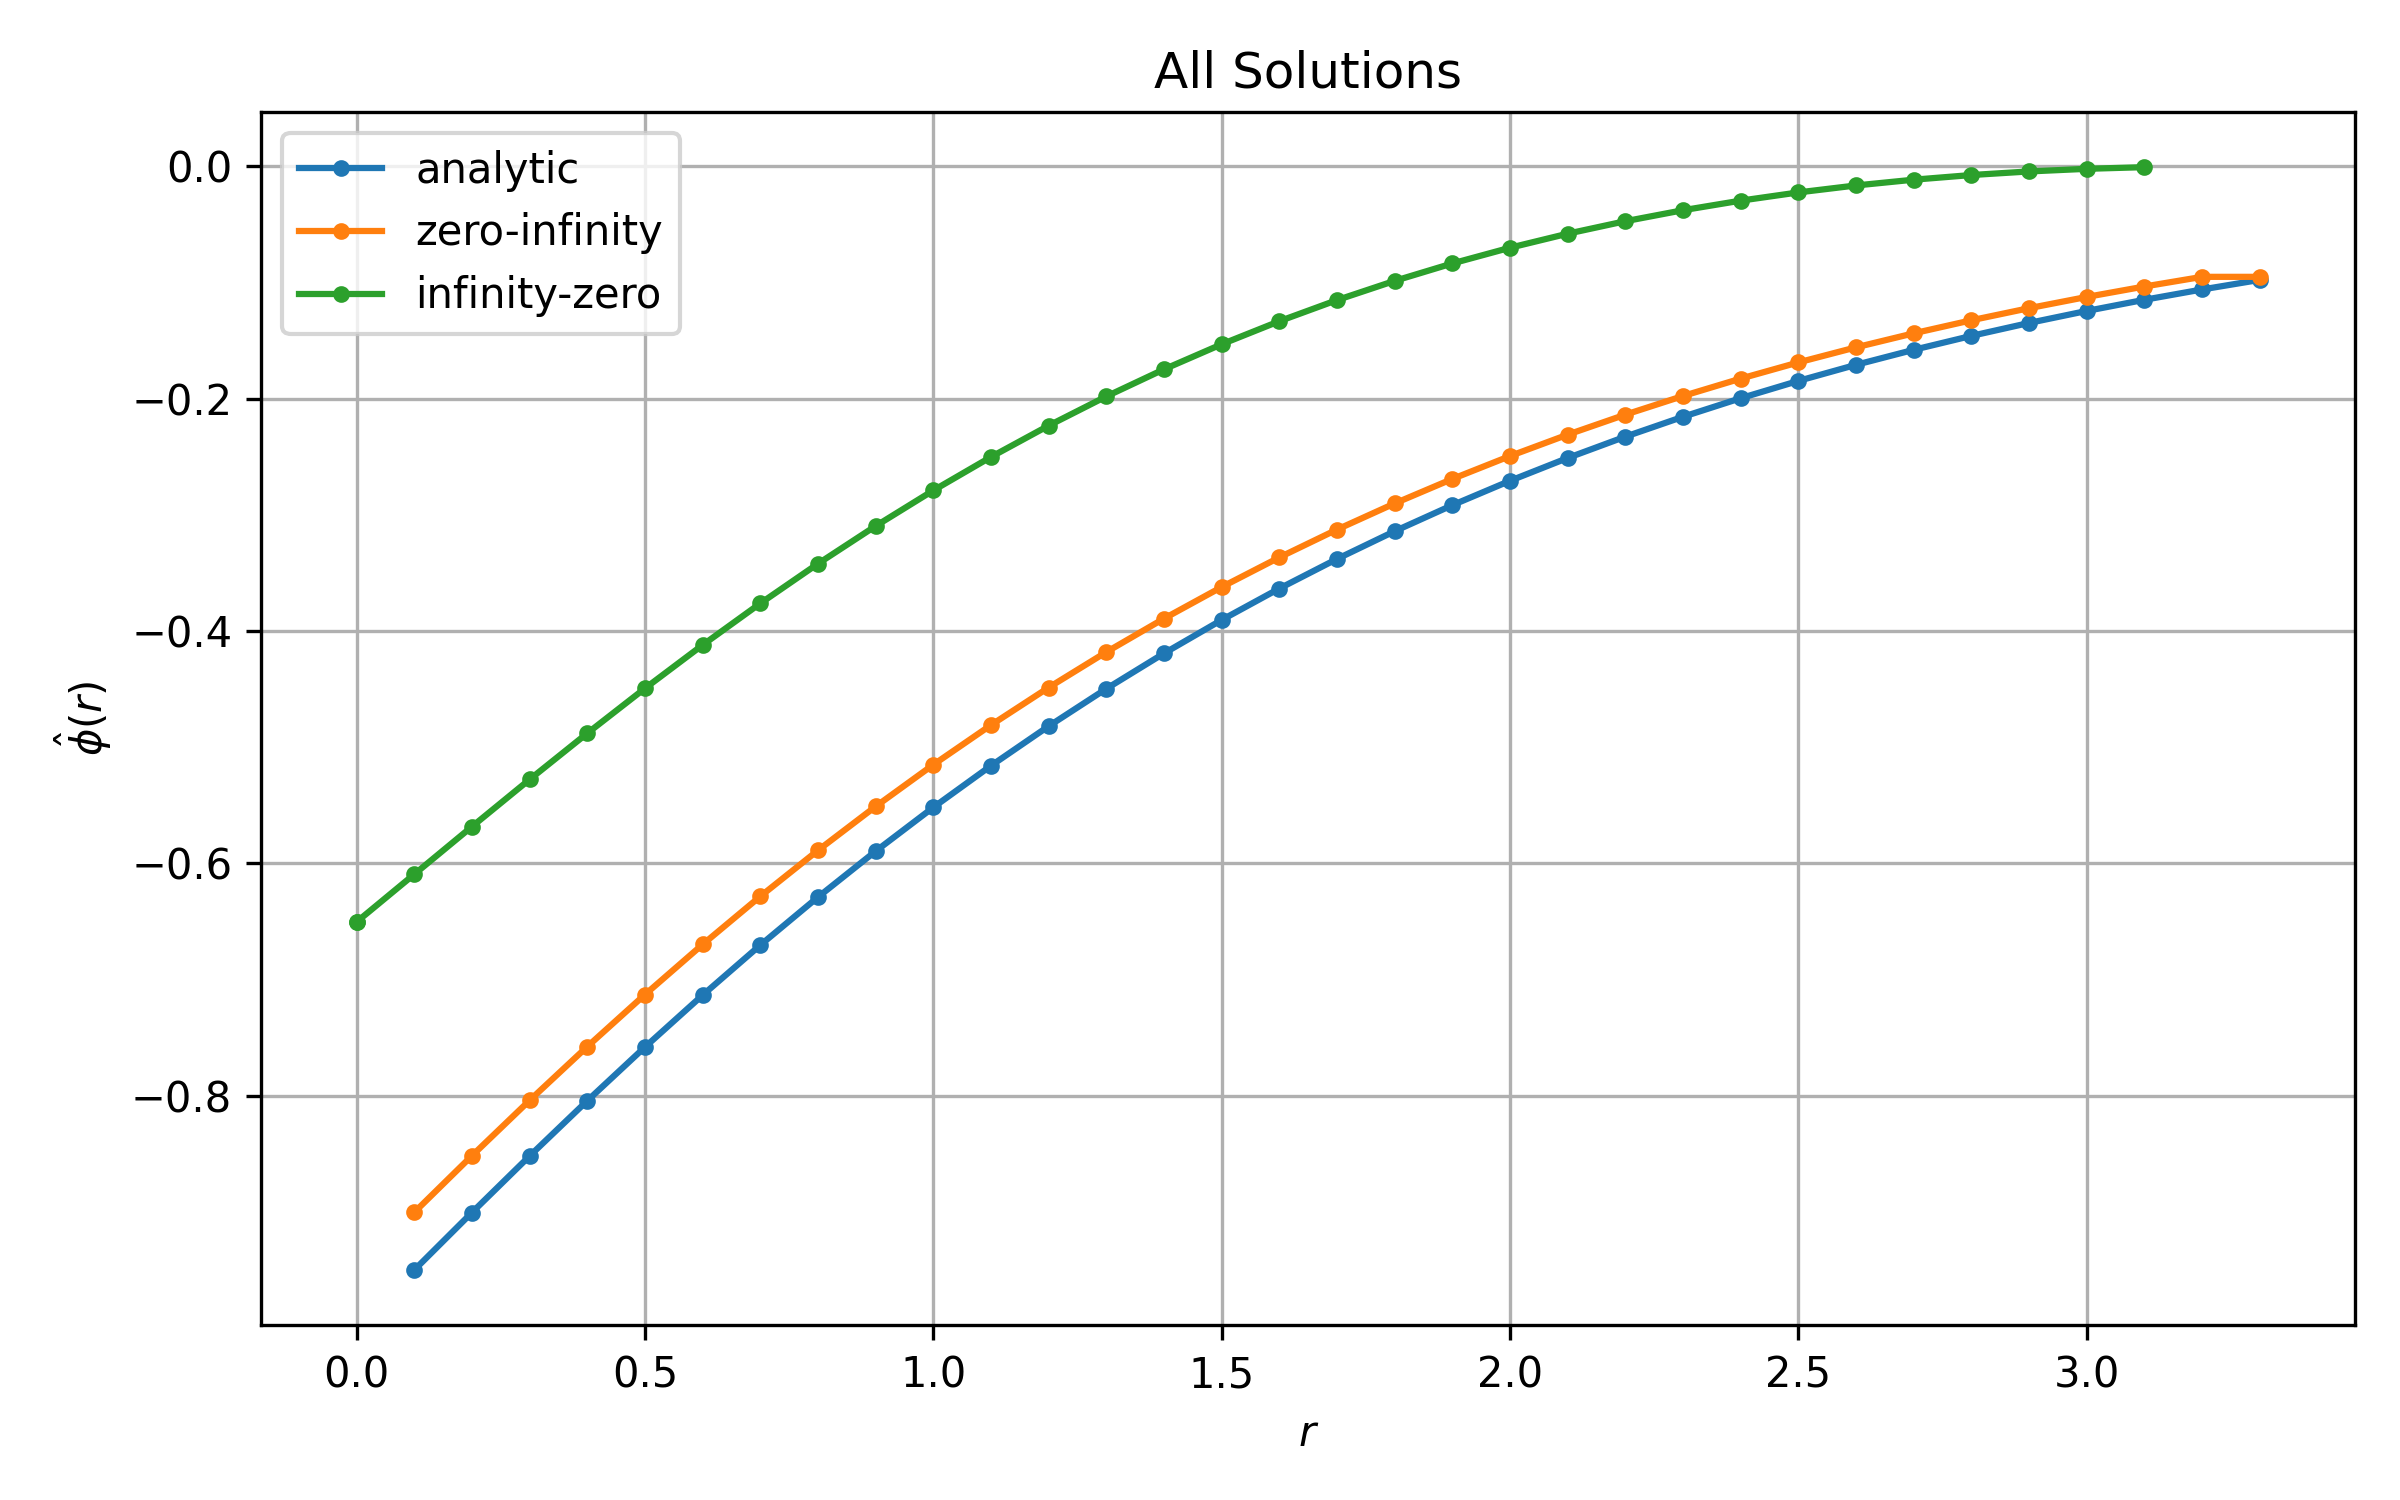
\includegraphics[scale=0.7]{../images/all-plots-0.1.png}
            \caption{Resultados para $\delta r = 0.1$}
            \label{fig:all-plots-0.1}
        \end{figure}
        \begin{figure}[H]
            \centering
            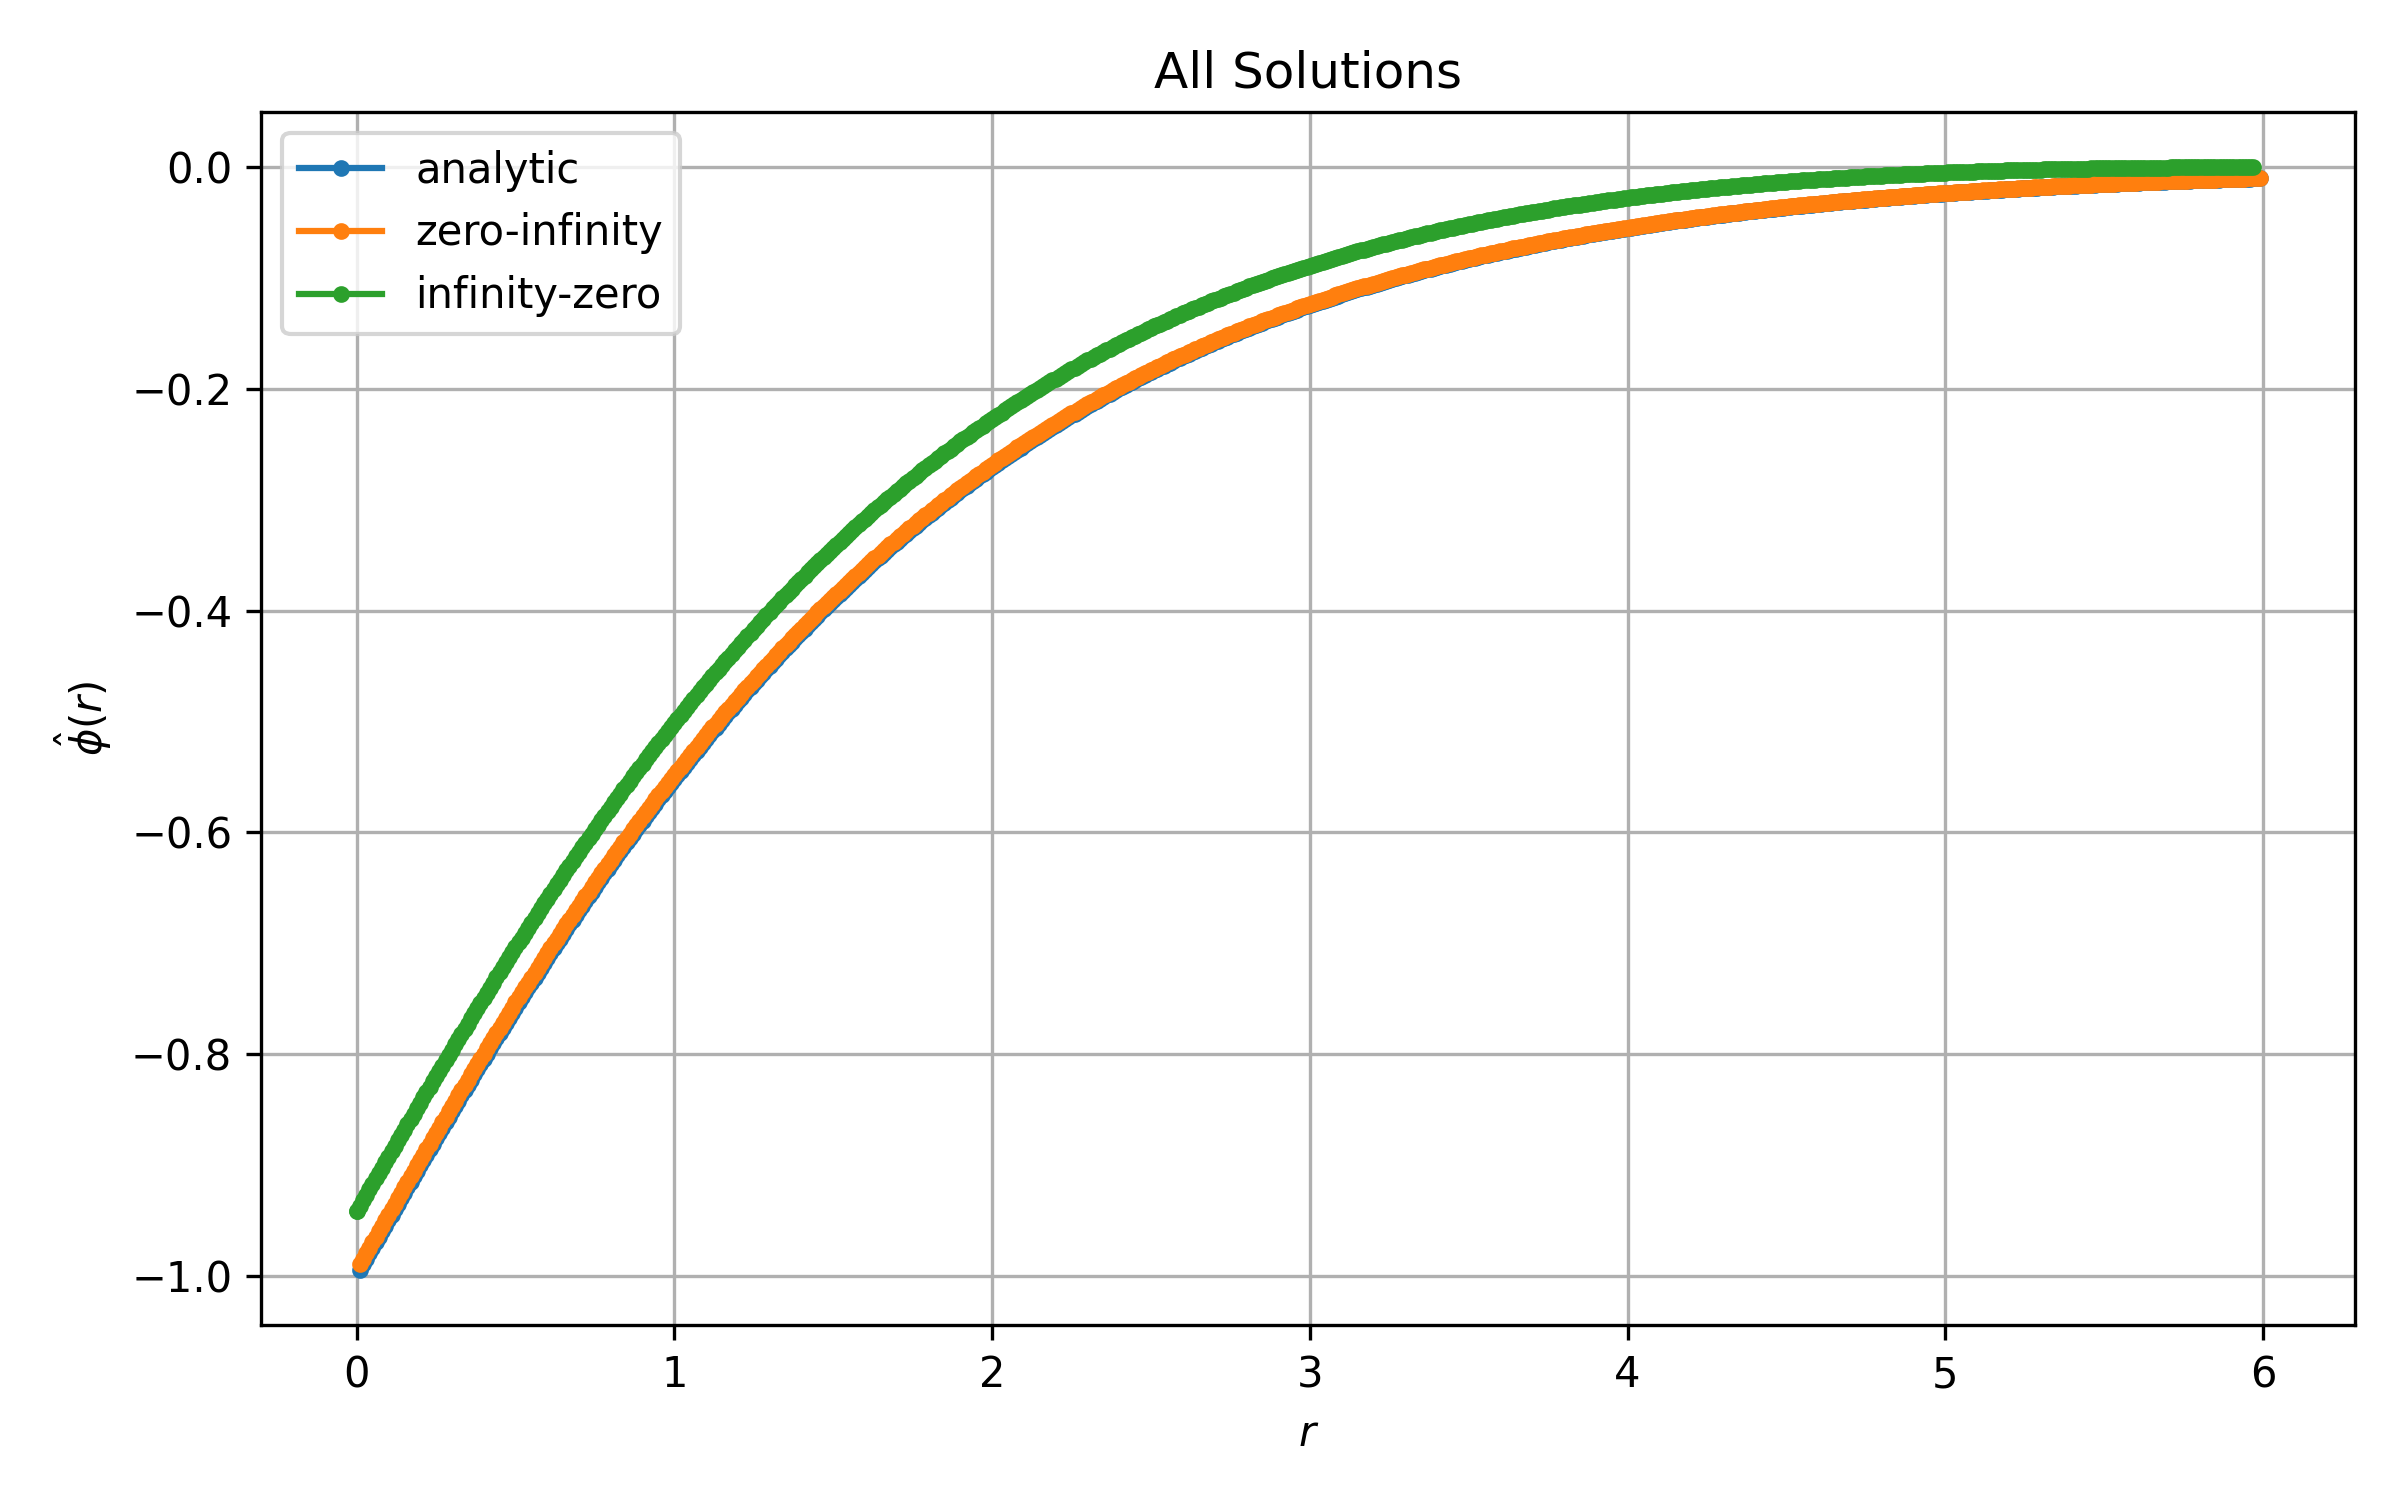
\includegraphics[scale=0.7]{../images/all-plots-0.01.png}
            \caption{Resultados para $\delta r = 0.01$}
            \label{fig:all-plots-0.01}
        \end{figure}
        \begin{figure}[H]
            \centering
            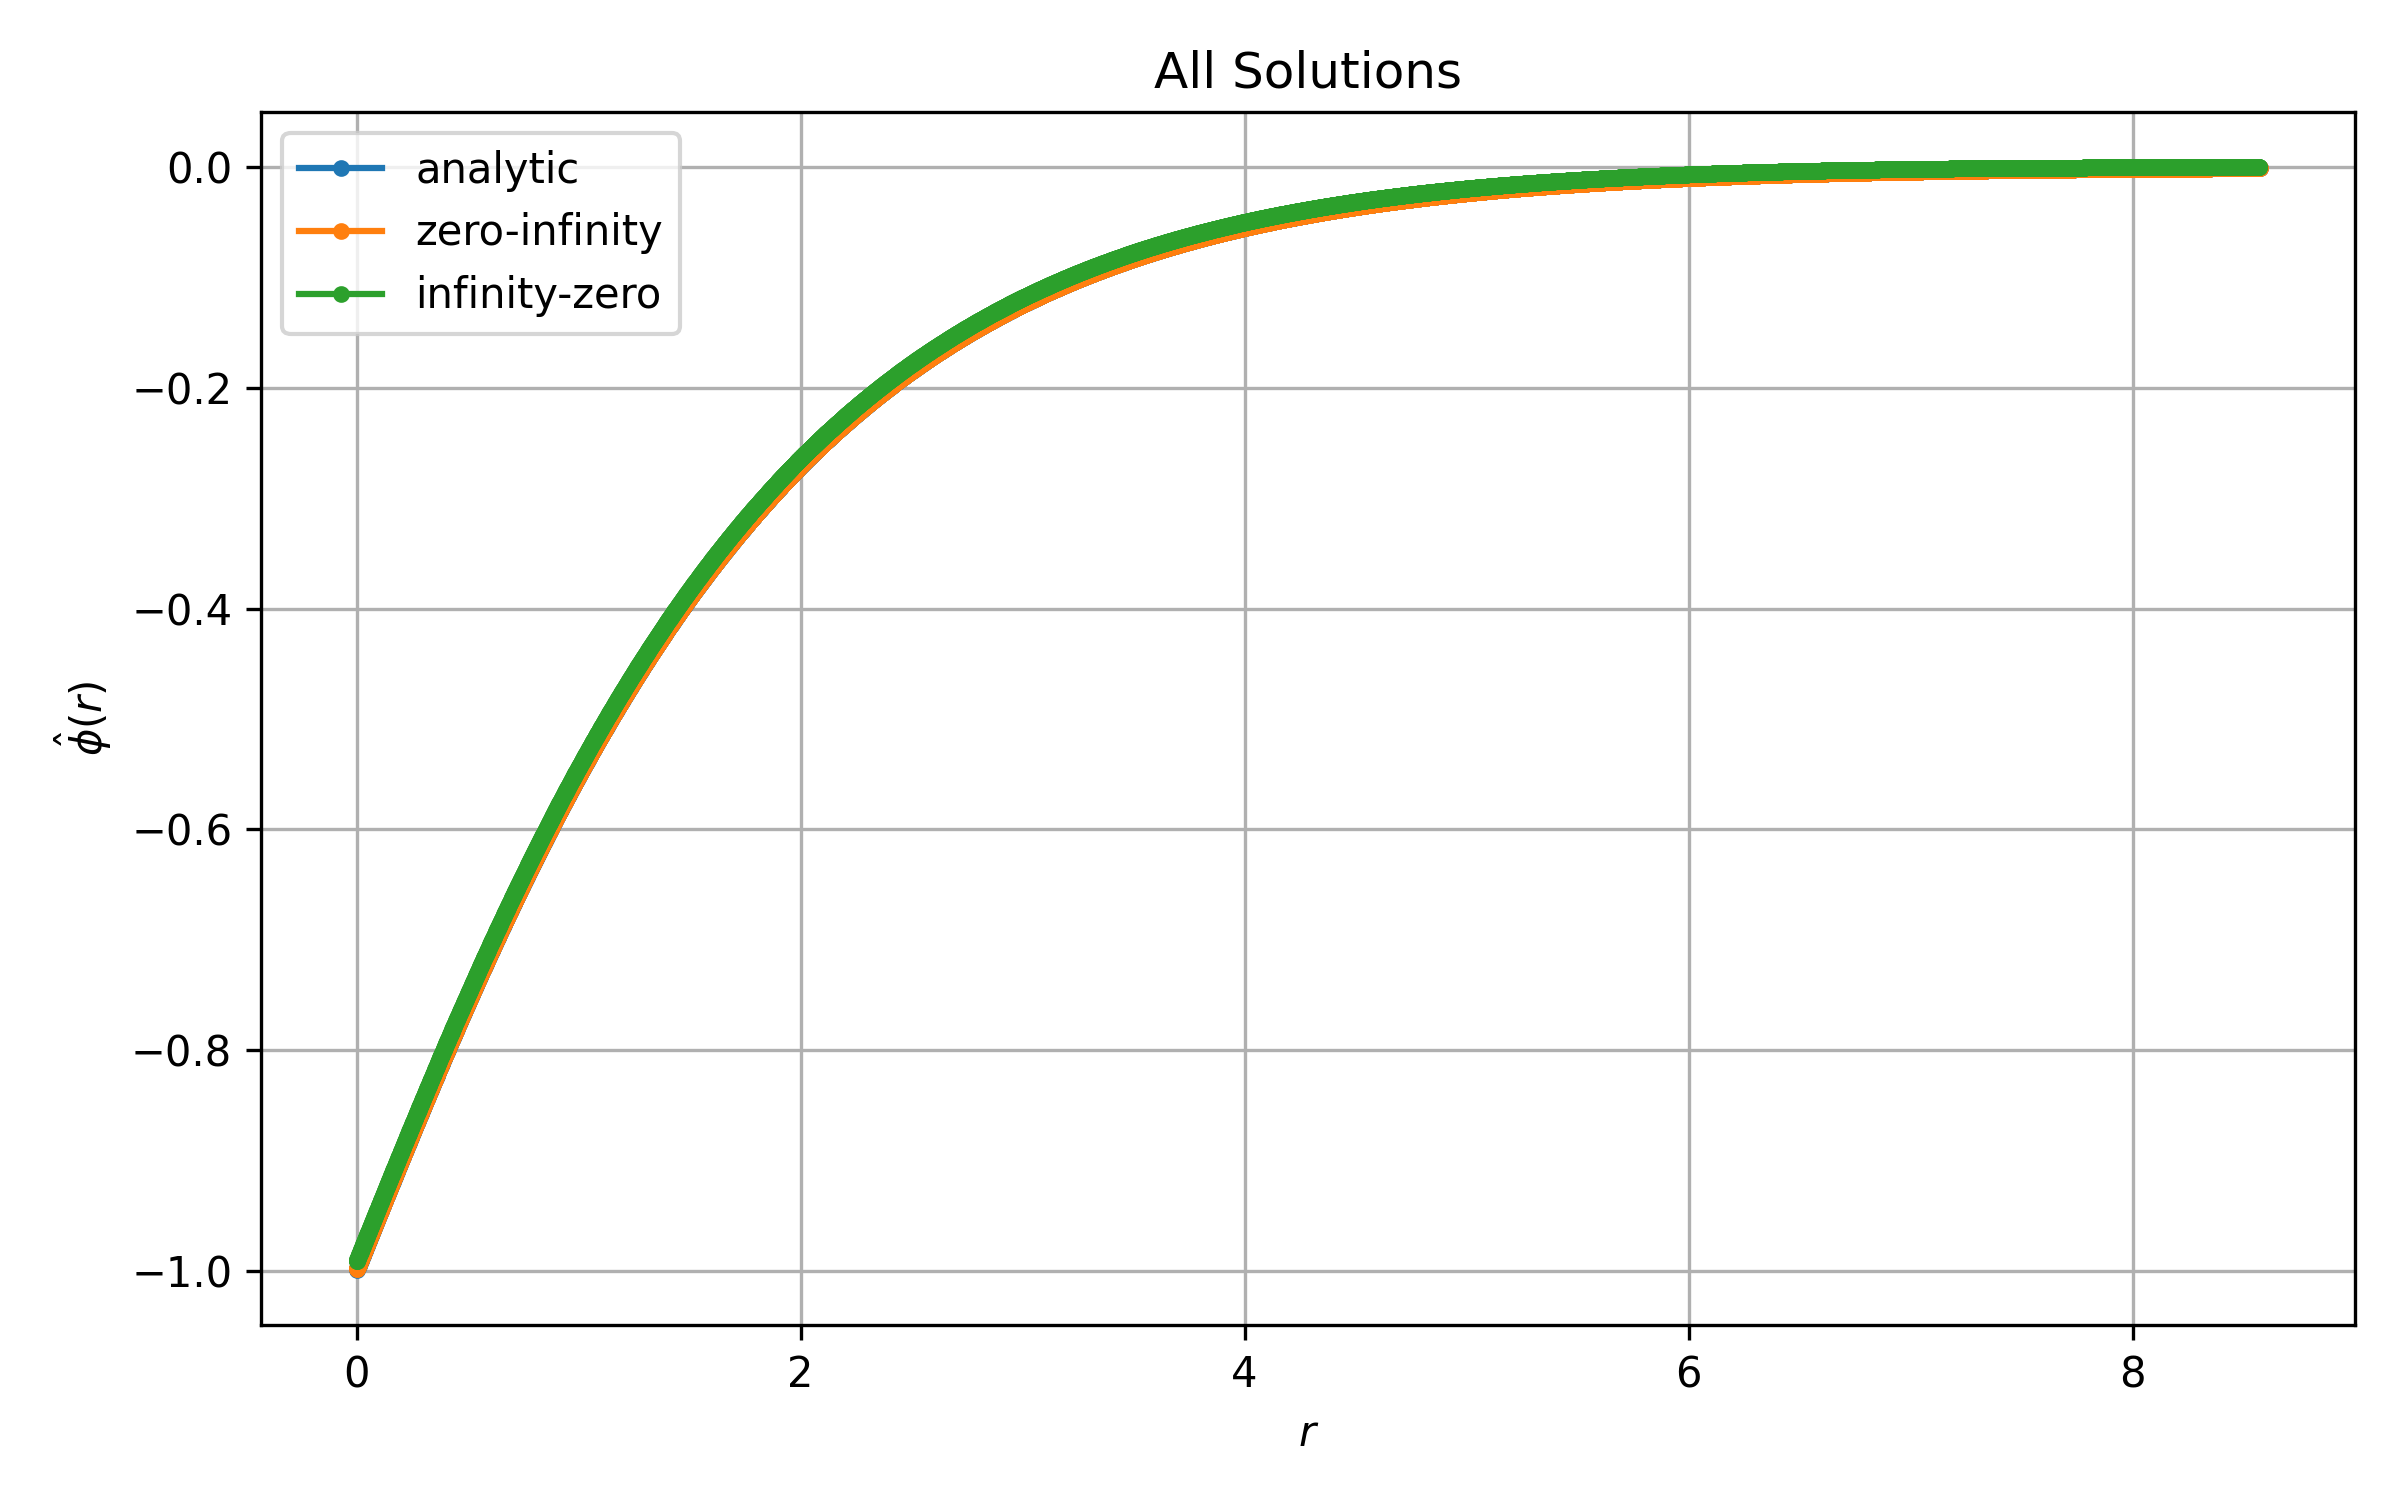
\includegraphics[scale=0.7]{../images/all-plots-0.001.png}
            \caption{Resultados para $\delta r = 0.001$}
            \label{fig:all-plots-0.001}
        \end{figure}
        \begin{figure}[H]
            \centering
            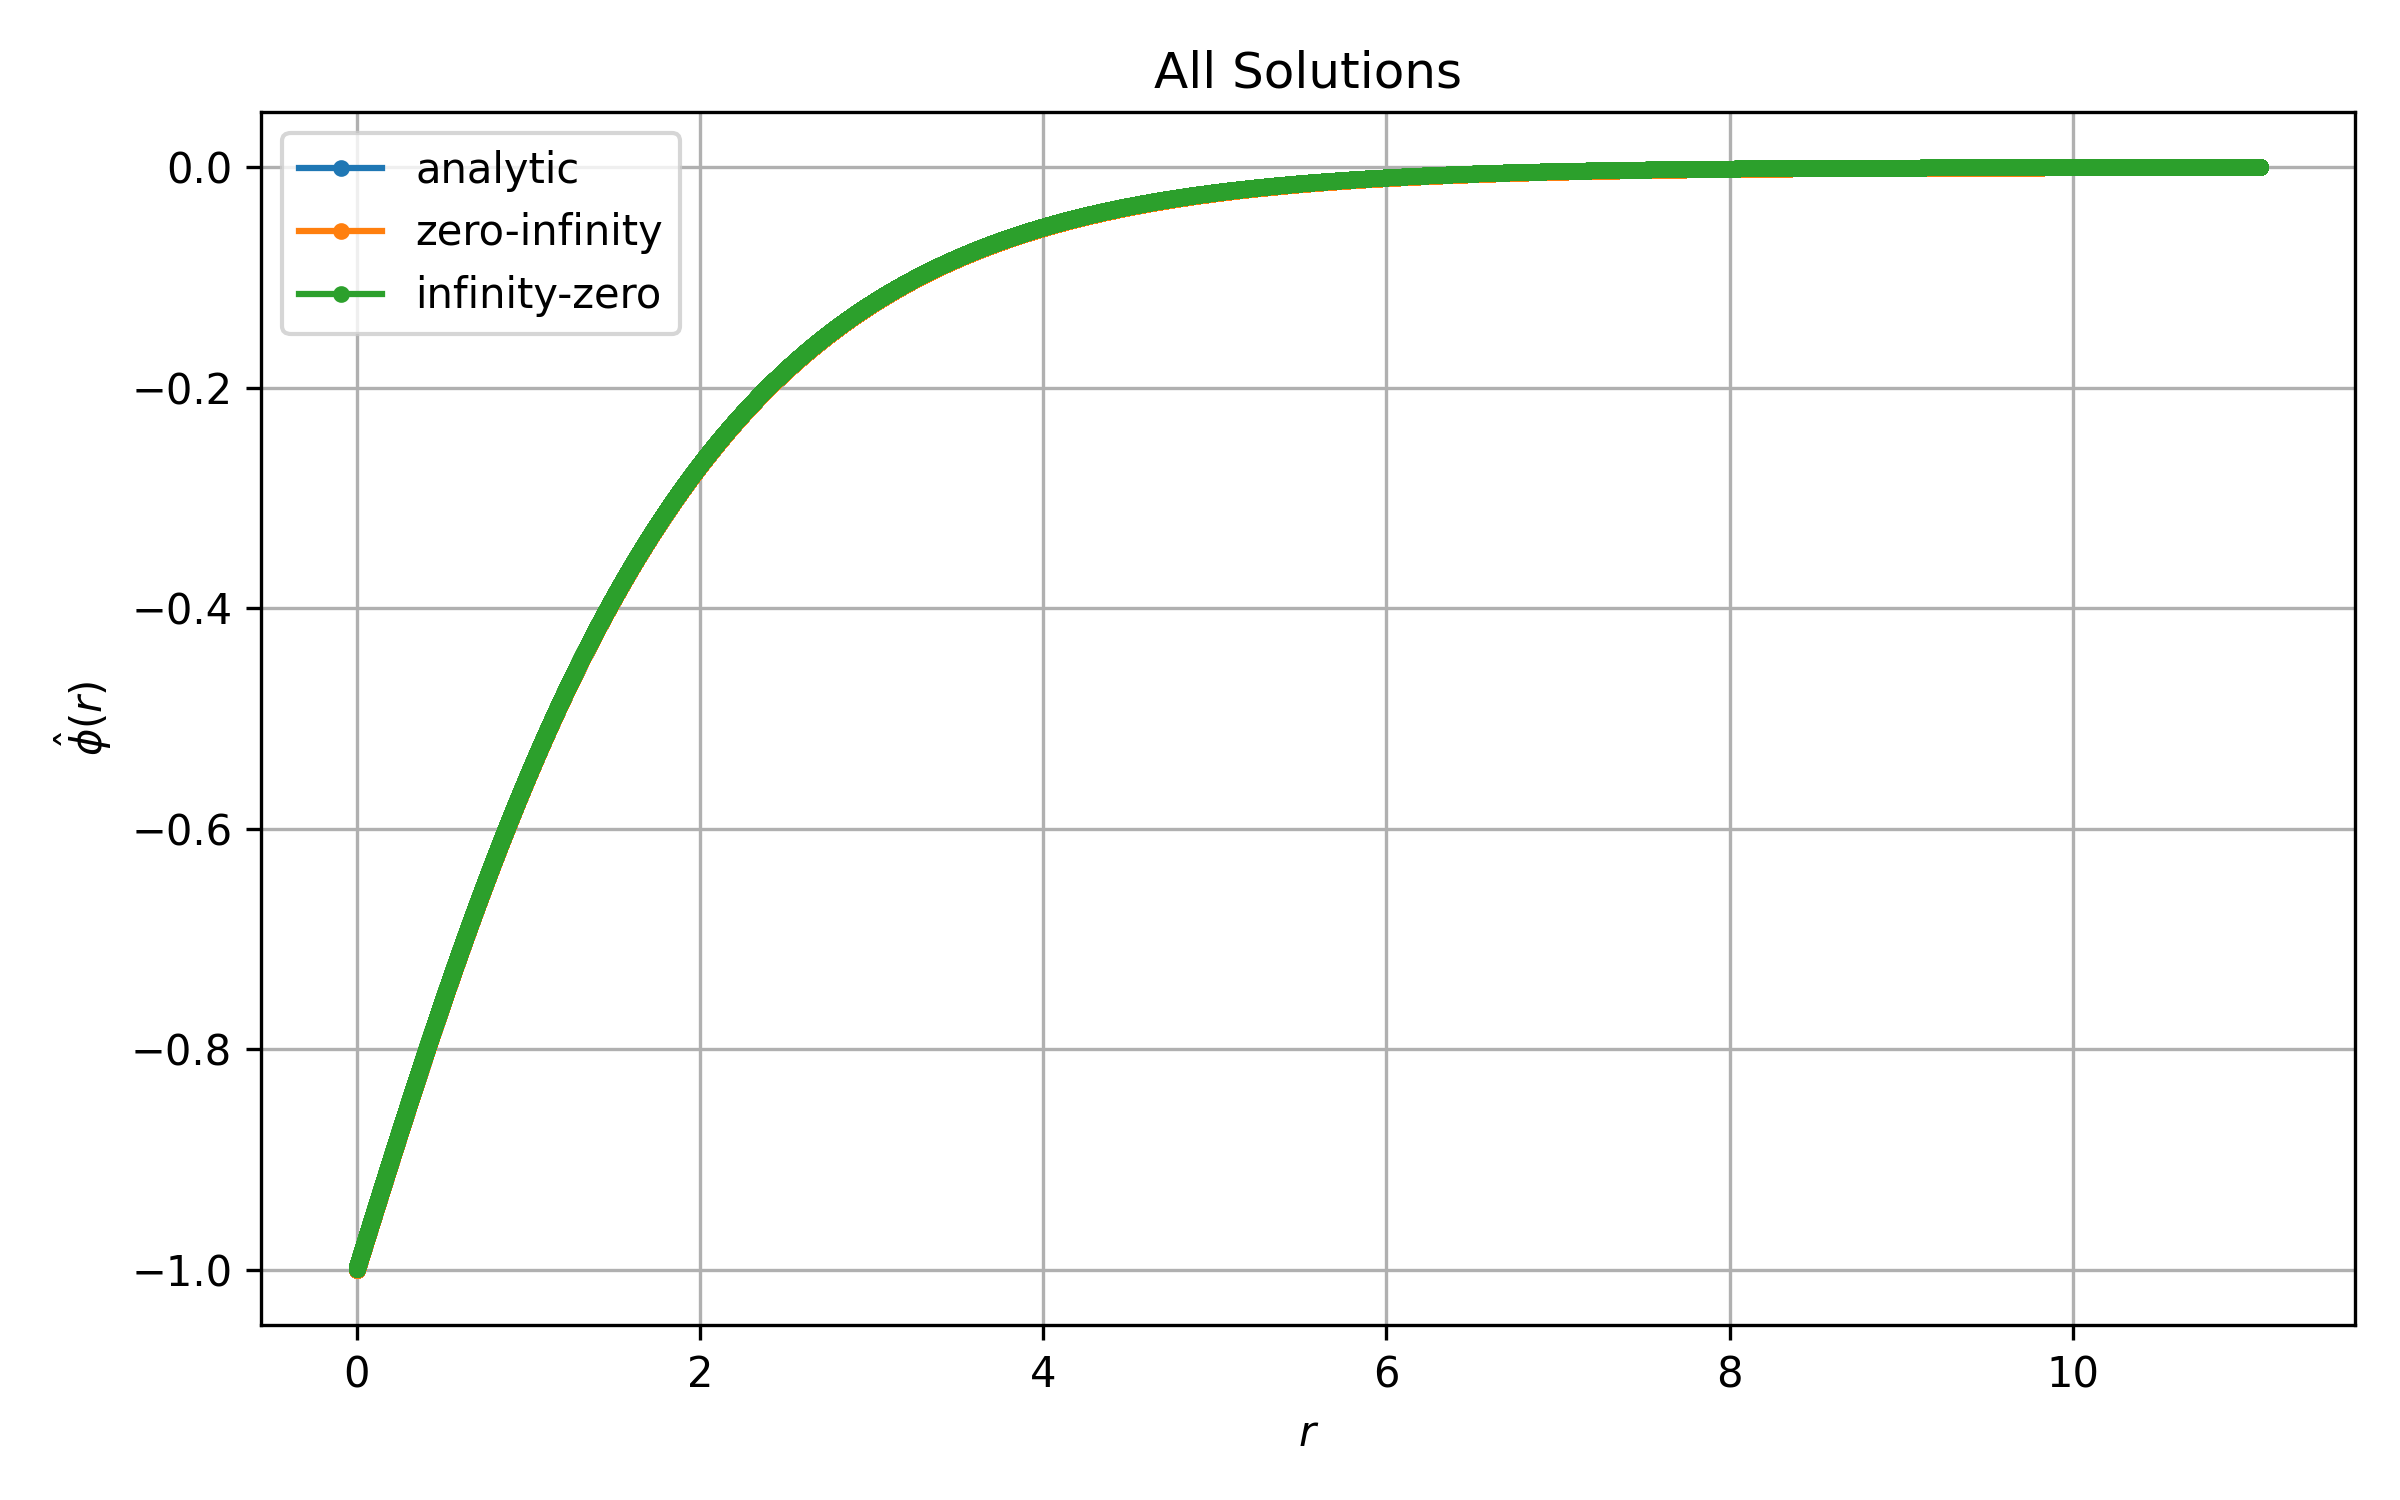
\includegraphics[scale=0.7]{../images/all-plots-0.0001.png}
            \caption{Resultados para $\delta r = 0.0001$}
            \label{fig:all-plots-0.0001}
        \end{figure}
        \begin{figure}[H]
            \centering
            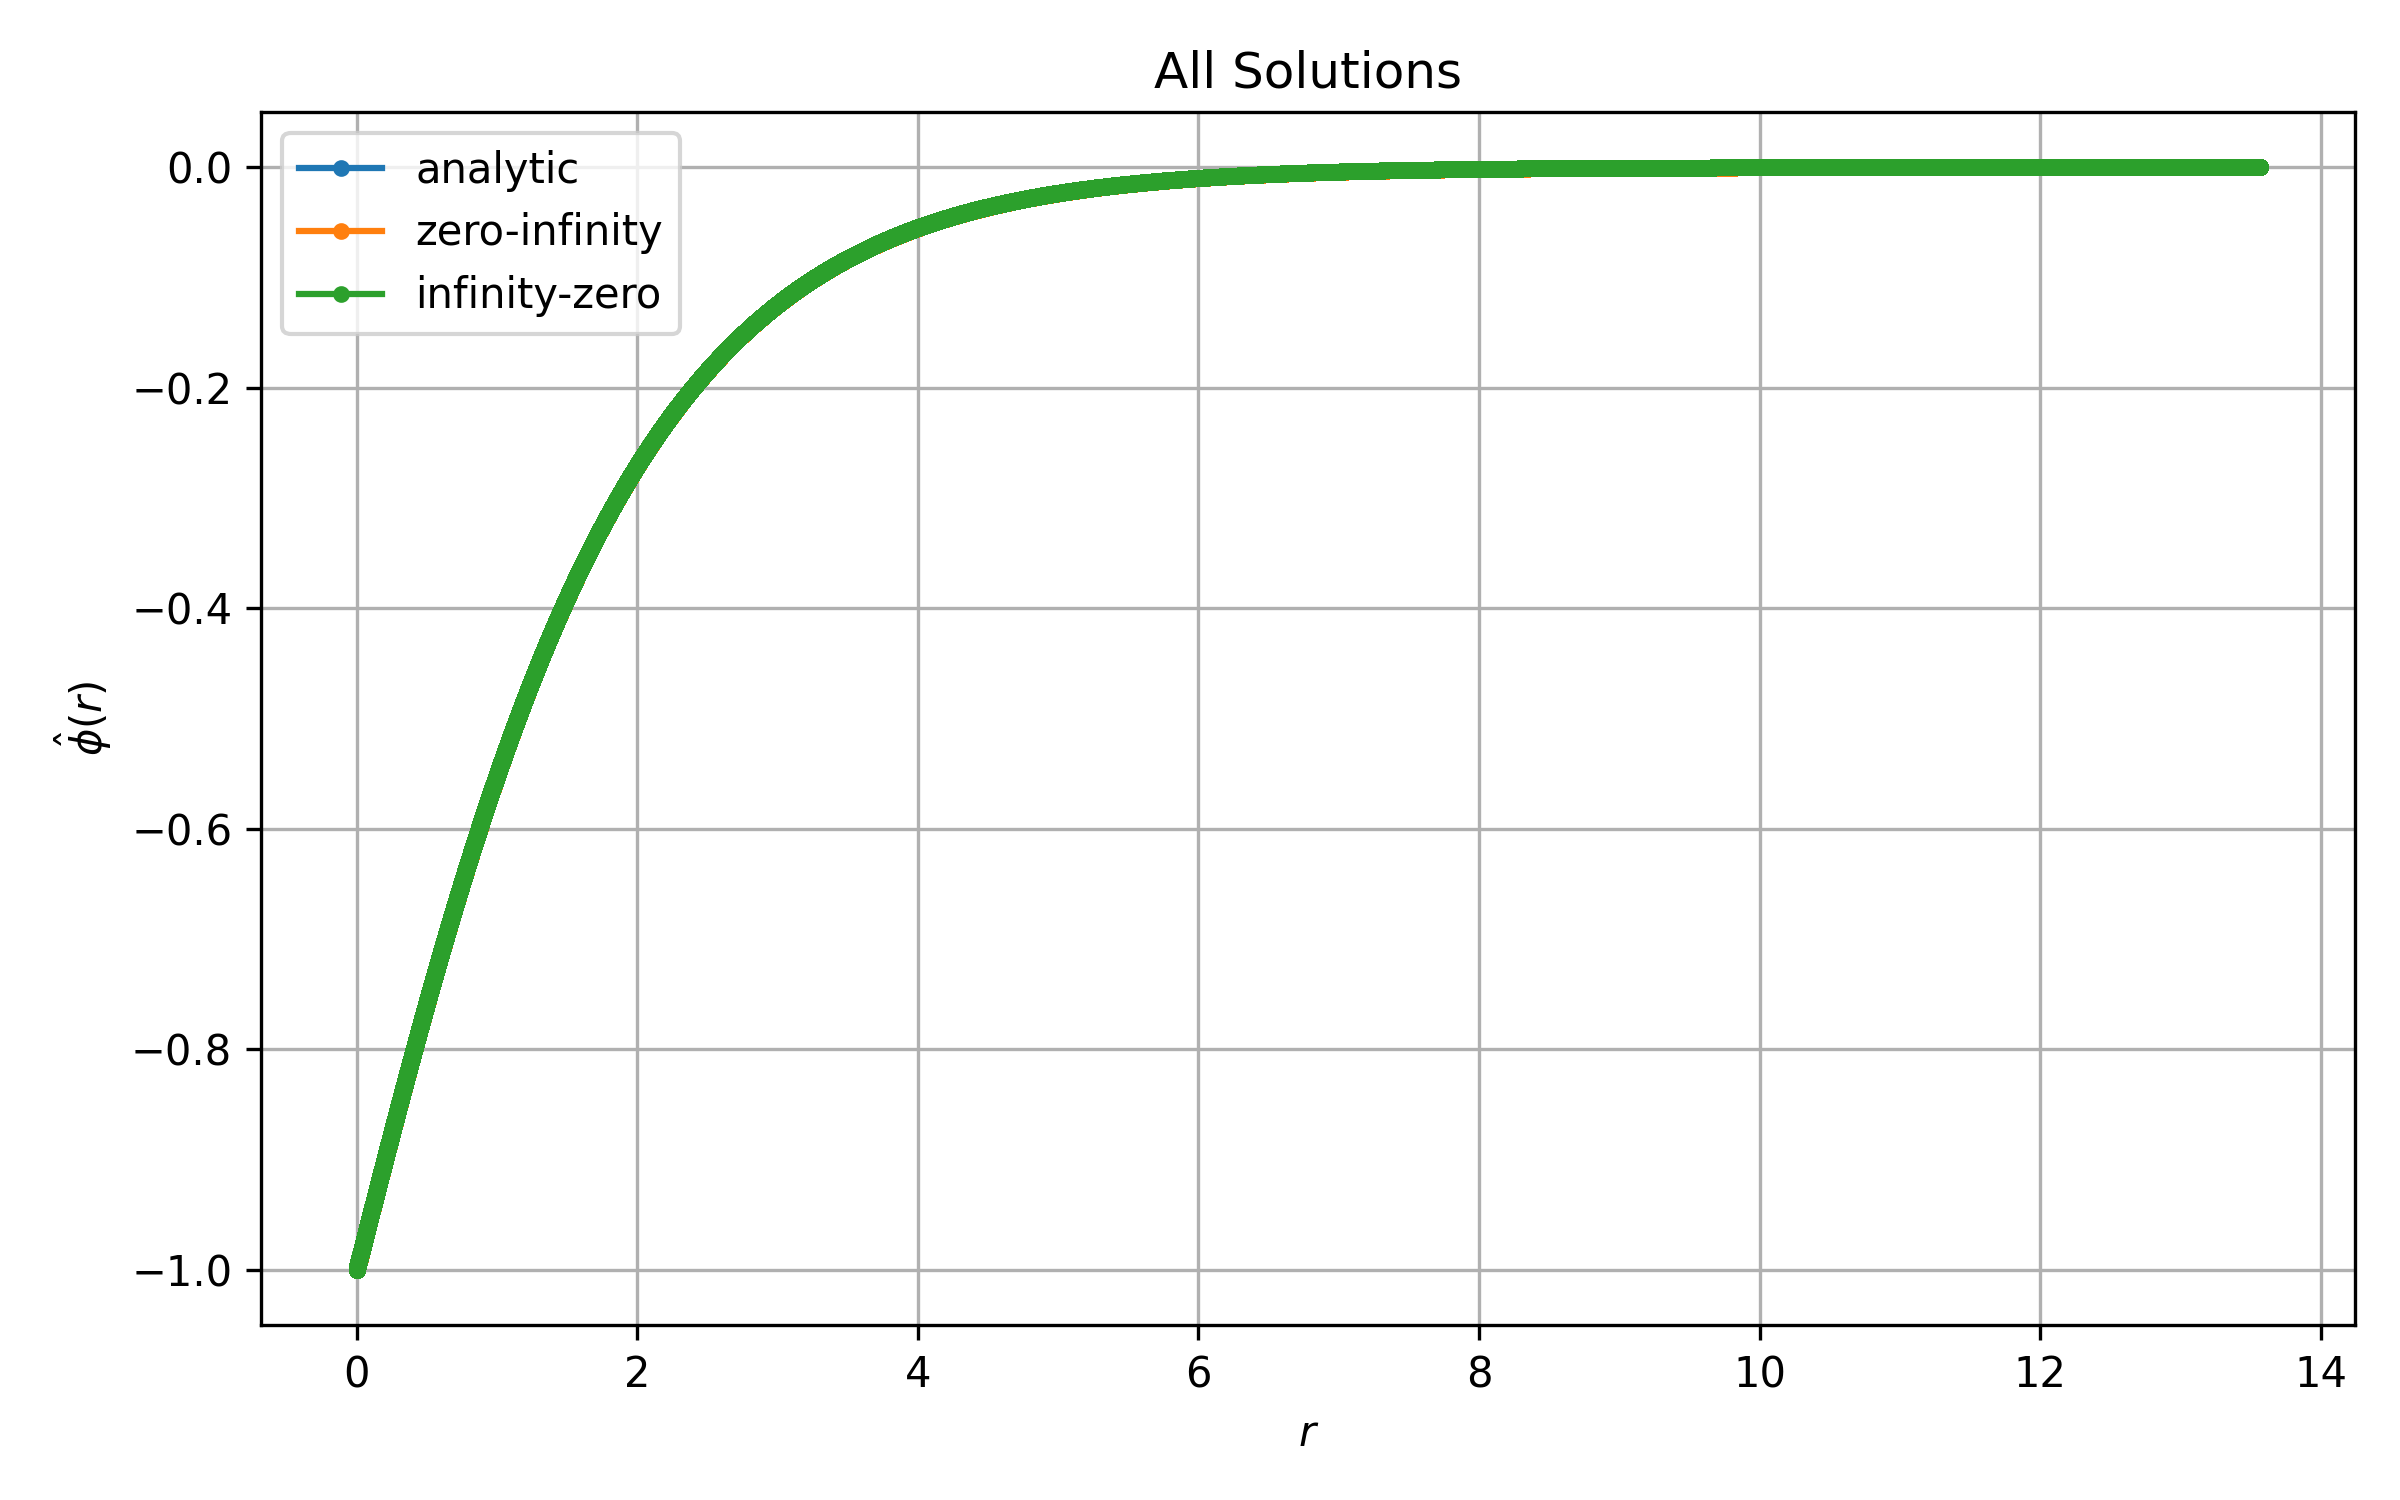
\includegraphics[scale=0.7]{../images/all-plots-1e-05.png}
            \caption{Resultados para $\delta r = 0.00001$}
            \label{fig:all-plots-0.00001}
        \end{figure}

        Analisando os gr\'aficos podemos ver que o m\'etodo de Numerov crescente converge mais rapidamente, ou seja, para valores maiores de $\delta r$ o algoritmo crescente se aproxima mais rapidamente da solu\c{c}\~ao anal\'itica. O mesmo n\~ao pode ser dito do algoritmo decrescente, que parece convergir apenas para valores muito pequenos de $\delta r$.

\section{The Matching Method}

        Considerar-se-a o potencial de Lennard-Jones, dado por:

        \begin{equation*}
            V(r) = 4E_{0} \left[ \left( \frac{a}{r} \right)^{12} - \left( \frac{a}{r} \right)^{6} \right]
        \end{equation*}

        que claramente satifaz V(r) $\to$ 0 quando r $\to \infty$ e V(r) $\to$ $+ \infty$ quando r $\to 0$. Ent\~ao, para estado ligado (E \textless  0) a solu\c{c}\~ao da equa\c{c}\~ao de Schr\"odinger com este potencial deve ser nula em r = 0 e r $\to \infty$. Assim, podemos resolv\^ela pelo m\'etodo de Numerov e pelo Matching Method.

        \subsection{Exerc\'icio 2}

            Tarefa: Encontrar analiticamente o ponto, $r_{0}$, de m\'inimo do potencial.

            Para simplificar a equa\c{c}\~ao, podemos definir $x = \frac{a}{r}$, assim temos que:
            \begin{equation*}
                V(x) = 4E_{0} \left[ x^{-12} - x^{-6} \right]
            \end{equation*}

            Para encontrar o ponto de m\'inimo do potencial, devemos derivar a equa\c{c}\~ao do potencial e igualar a zero:
            \begin{equation*}
                \frac{dV(x)}{dx} = 0
            \end{equation*}
            Derivando a equa\c{c}\~ao do potencial, obtemos:
            \begin{equation*}
                \frac{dV(x)}{dx} = 4E_{0} \left[ -12{x}^{-13} + 6{x}^{-7} \right]
            \end{equation*}
            Igualando a zero, obtemos:
            \begin{equation*}
                0 = -12{x}^{-13} + 6{x}^{-7}
            \end{equation*}
            Assim, temos que:
            \begin{equation*}
                2{x}^{-6} = 1
            \end{equation*}
            Por fim, isolando x, obtemos:
            \begin{equation*}
                x_{0} = 2^{1/6}
            \end{equation*}
            Devemos verificar se este ponto \'e realmente um m\'inimo, para isso devemos derivar a equa\c{c}\~ao do potencial novamente e verificar se o resultado \'e positivo:
            \begin{equation*}
                \frac{d^{2}V(x)}{dx^{2}} = 4E_{0} \left[ 156{x}^{-14} - 42{x}^{-8} \right]
            \end{equation*}
            Calculando a segunda derivada no ponto $x_{0}$, obtemos:
            \begin{equation*}
                \frac{d^{2}V(x_{0})}{dx^{2}} = 4E_{0} \left[ 156(2^{1/6})^{-14} - 42(2^{1/6})^{-8} \right]
            \end{equation*}
            Assim, temos que:
            \begin{equation*}
                \frac{d^{2}V(x_{0})}{dx^{2}} = 4E_{0} \left[ 156(2^{-14/6}) - 42(2^{-8/6}) \right]
            \end{equation*}
            Que \'e aproximadamente:
            \begin{equation*}
                \frac{d^{2}V(x_{0})}{dx^{2}} \approx 57.14E_{0}
            \end{equation*}
            Como $E_{0}$ \'e positivo, temos que:
            \begin{equation*}
                \frac{d^{2}V(x_{0})}{dx^{2}} > 0
            \end{equation*}
            Portanto, o ponto $x_{0}$ \'e realmente um m\'inimo do potencial.
        
        \subsection{Exerc\'icio 3}

            Tarefa: Utilizar o Matching Method para encontrar os autovalores e autoestados da equa\c{c}\~ao de Schr\"oedinger com potencial de Lennard-Jones dado dois valores de $E_{0}$ diferentes.

            A equa\c{c}\~ao de Schr\"odinger \'e dada por:
            \begin{equation*}
                -\frac{\hbar^{2}}{2m} \frac{d^{2}\psi(r)}{dr^{2}} + 4E_{0} \left[ \left( \frac{r}{a} \right)^{-12} - \left( \frac{r}{a} \right)^{-6} \right]\psi(r) = E\psi(r)
            \end{equation*}
            supondo simetria esf\'erica.

            Faz-se $x = \frac{r}{a}$:
            \begin{equation*}
                -\frac{\hbar^{2}}{2ma^2} \frac{d^{2}\psi(x)}{dx^{2}} + 4E_{0} \left[ x^{-12} - x^{-6} \right]\psi(x) = E\psi(x)
            \end{equation*}

            Note que $\frac{\hbar^{2}}{2ma^2}$ tem dimens\~ao de energia, e portanto define-se $k = \frac{2Ema^2}{\hbar^{2}}$ e $k' = \frac{8E_{0}ma^2}{\hbar^{2}}$. Assim, temos que:
            \begin{equation*}
                \frac{d^{2}\psi(x)}{dx^{2}} - k'\left[  x^{-12} - x^{-6} \right]\psi(x) = -k\psi(x)
            \end{equation*}

            E por fim, rearranja-se a equa\c{c}\~ao:
            \begin{equation*}
                \frac{d^{2}\psi(x)}{dx^{2}} = \left[k'\left( x^{-12} - x^{-6} \right) -k\right]\psi(x)
            \end{equation*}

            Para simplificar, adota-se $E_{0_{1}} = \frac{\hbar^{2}}{8ma^2}$ e $E_{0_{2}} = 2\frac{\hbar^{2}}{8ma^2}$ de modo que $k'_{1} = 750$ e $k'_{2} = 1000$.

            A energia mínima $E_{min}$ para que haja partícula \'e igual ao potencial em seu m\'inimo $V(r_{0}) = -2E_{0}$. Mas queremos expressar isto em termos de k' e k para representarmos no c\'odigo.
            
            Substituimos $E_{min}$ na expressão de k e obtemos:

            \begin{equation}
                k_{min} = \frac{2E_{min}ma^2}{\hbar^{2}} = - \frac{4E_{0}ma^2}{\hbar^{2}}
            \end{equation}

            E, utilizando a expressão para k', temos:

            \begin{equation}
                k_{min} = -\frac{k'}{2}
            \end{equation}

            E podemos partir deste m\'inimo para descobrir os k

            Assim, compilou-se o código com:

            gfortran P1-5255417-ex-3.f90 -Wall -Wextra -pedantic -o P1-5255417-ex-3.exe

            E executou-se o código com os seguintes parâmetros:
            \begin{figure}[H]
                \centering
                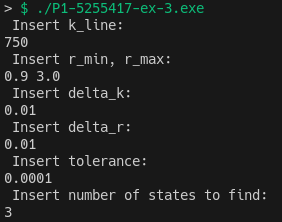
\includegraphics[scale=0.7]{../images/ex3-750-parameters.png}
                \caption{Par\^ametros para k' = 750}
            \end{figure}
            e tamb\'em com:
            \begin{figure}[H]
                \centering
                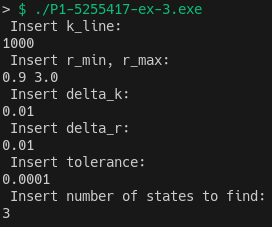
\includegraphics[scale=0.7]{../images/ex3-1000-parameters.png}
                \caption{Par\^ametros para k' = 1000}
            \end{figure}
              
            Abaixo, os gr\'aficos resultantes:

            \begin{figure}[H]
                \centering
                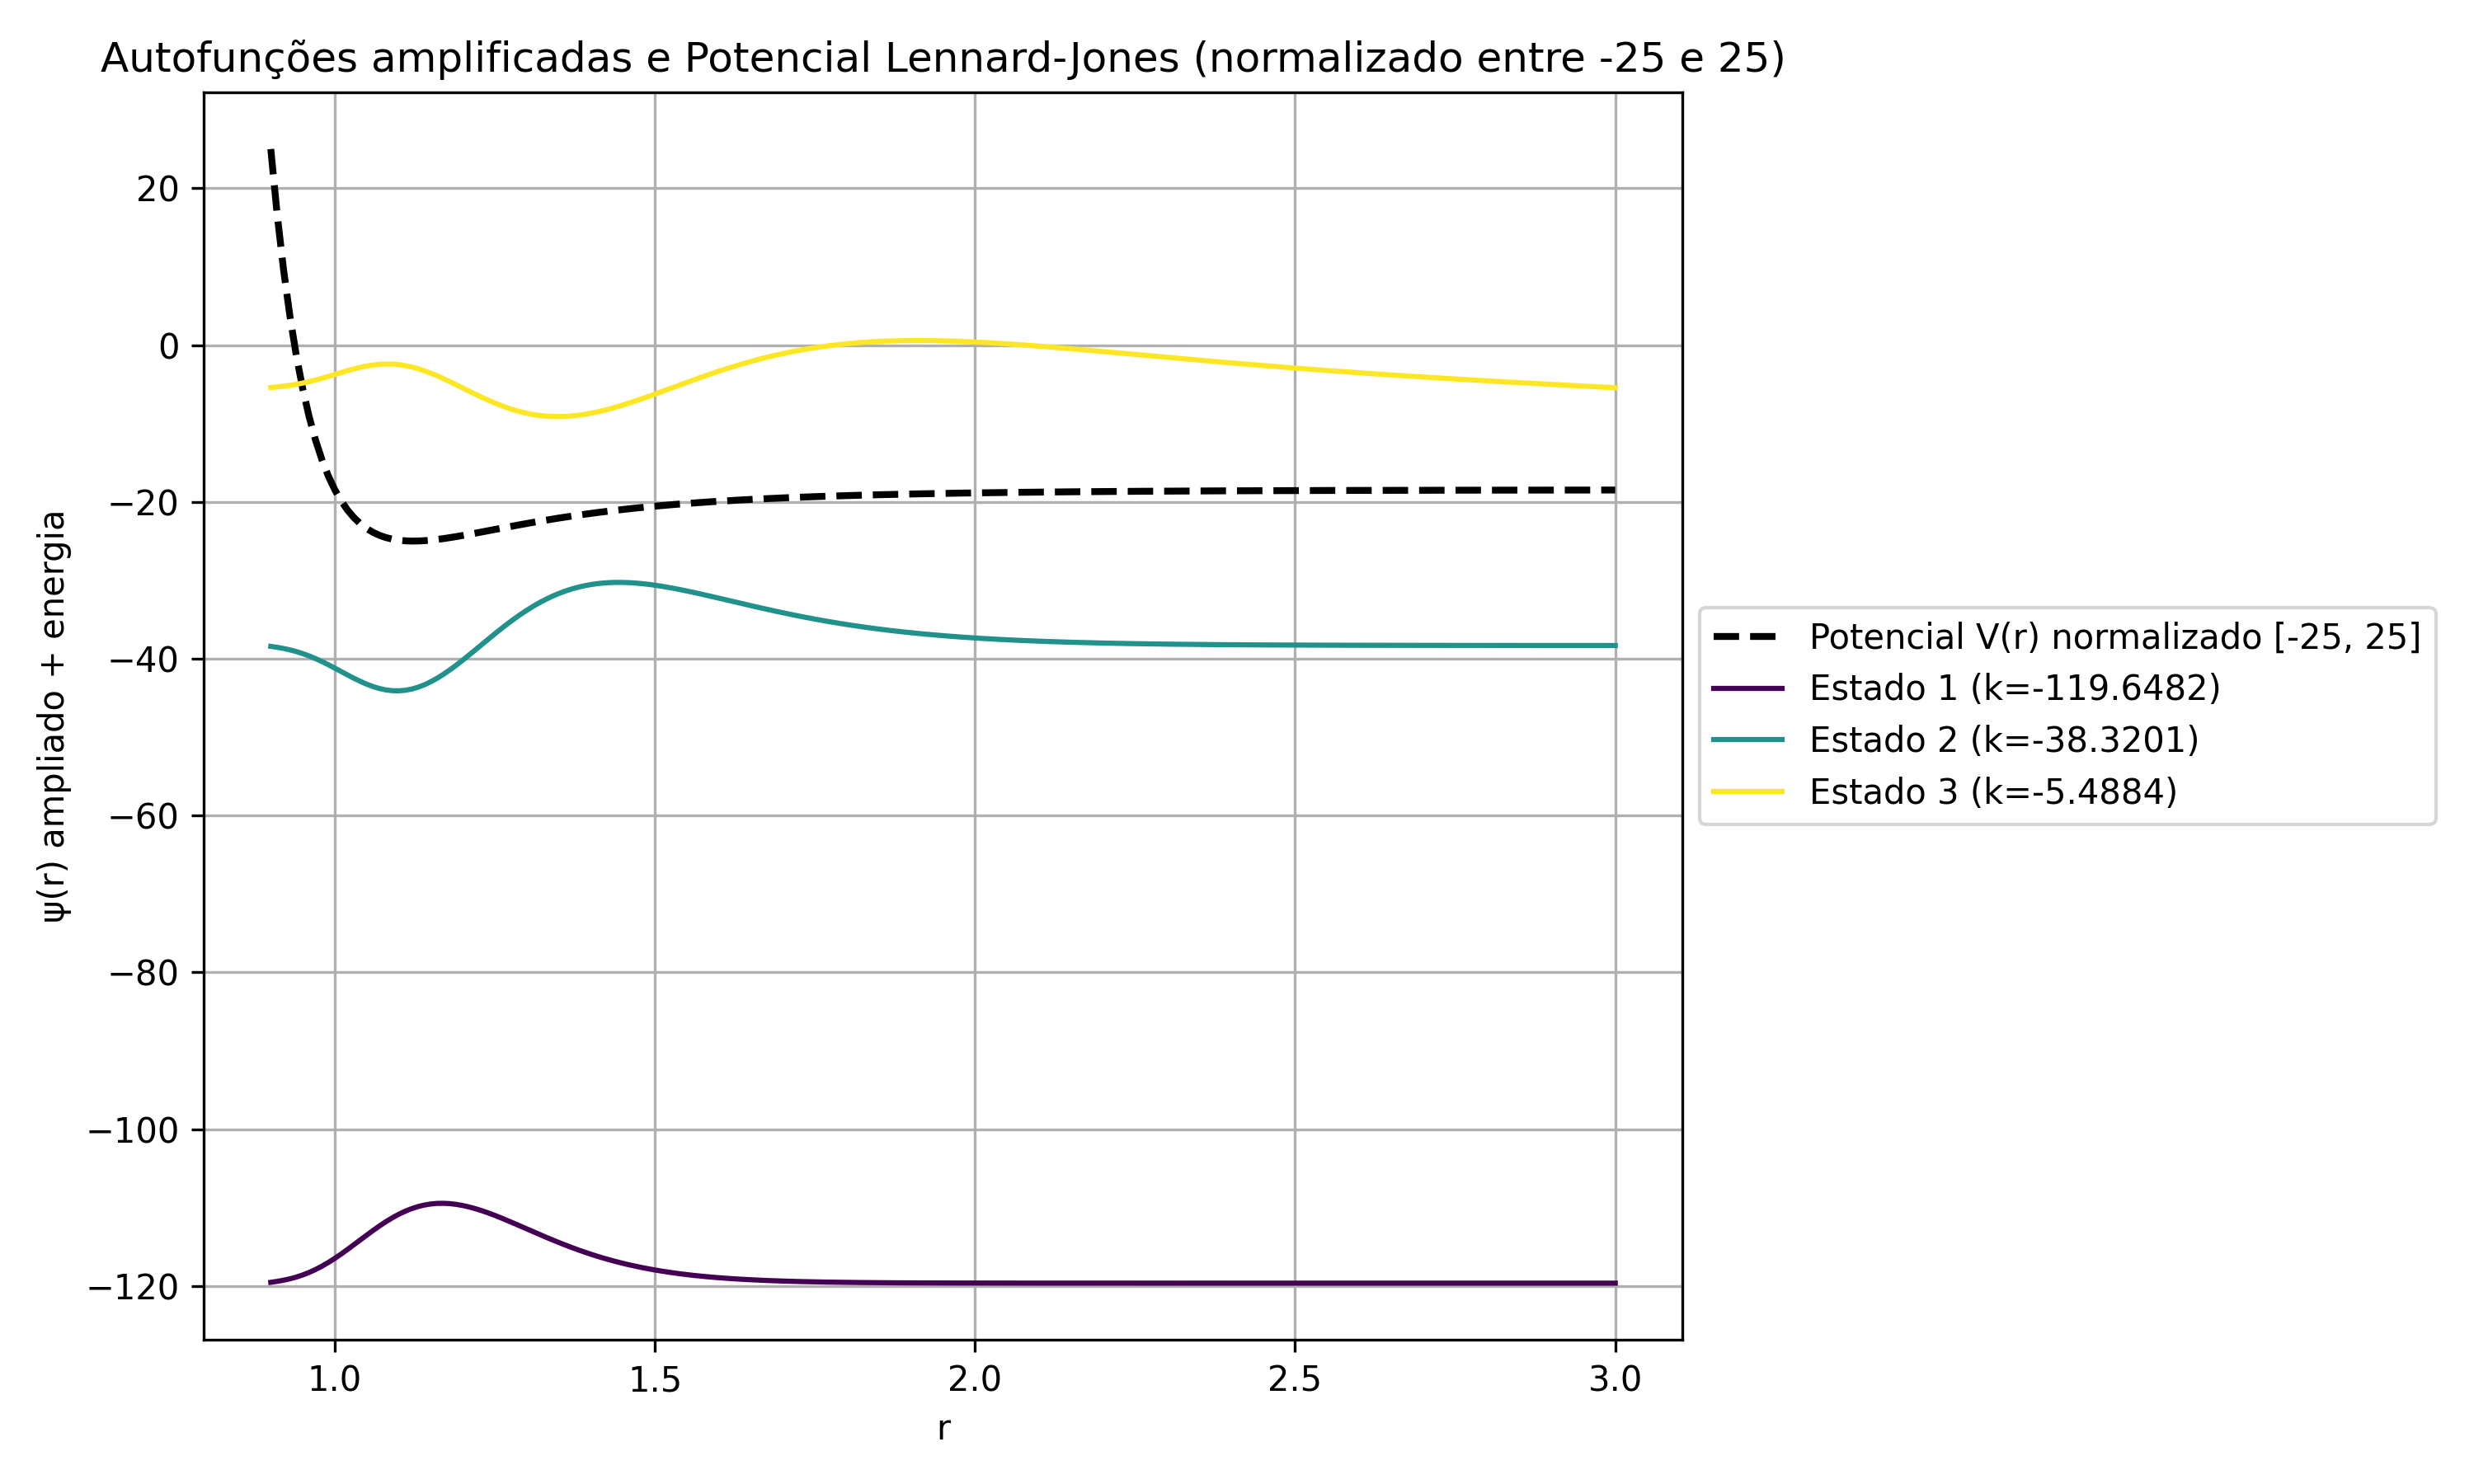
\includegraphics[scale=0.7]{../images/ex3-results-750.png}
                \caption{Resultados para k' = 750}
            \end{figure}
            \begin{figure}[H]
                \centering
                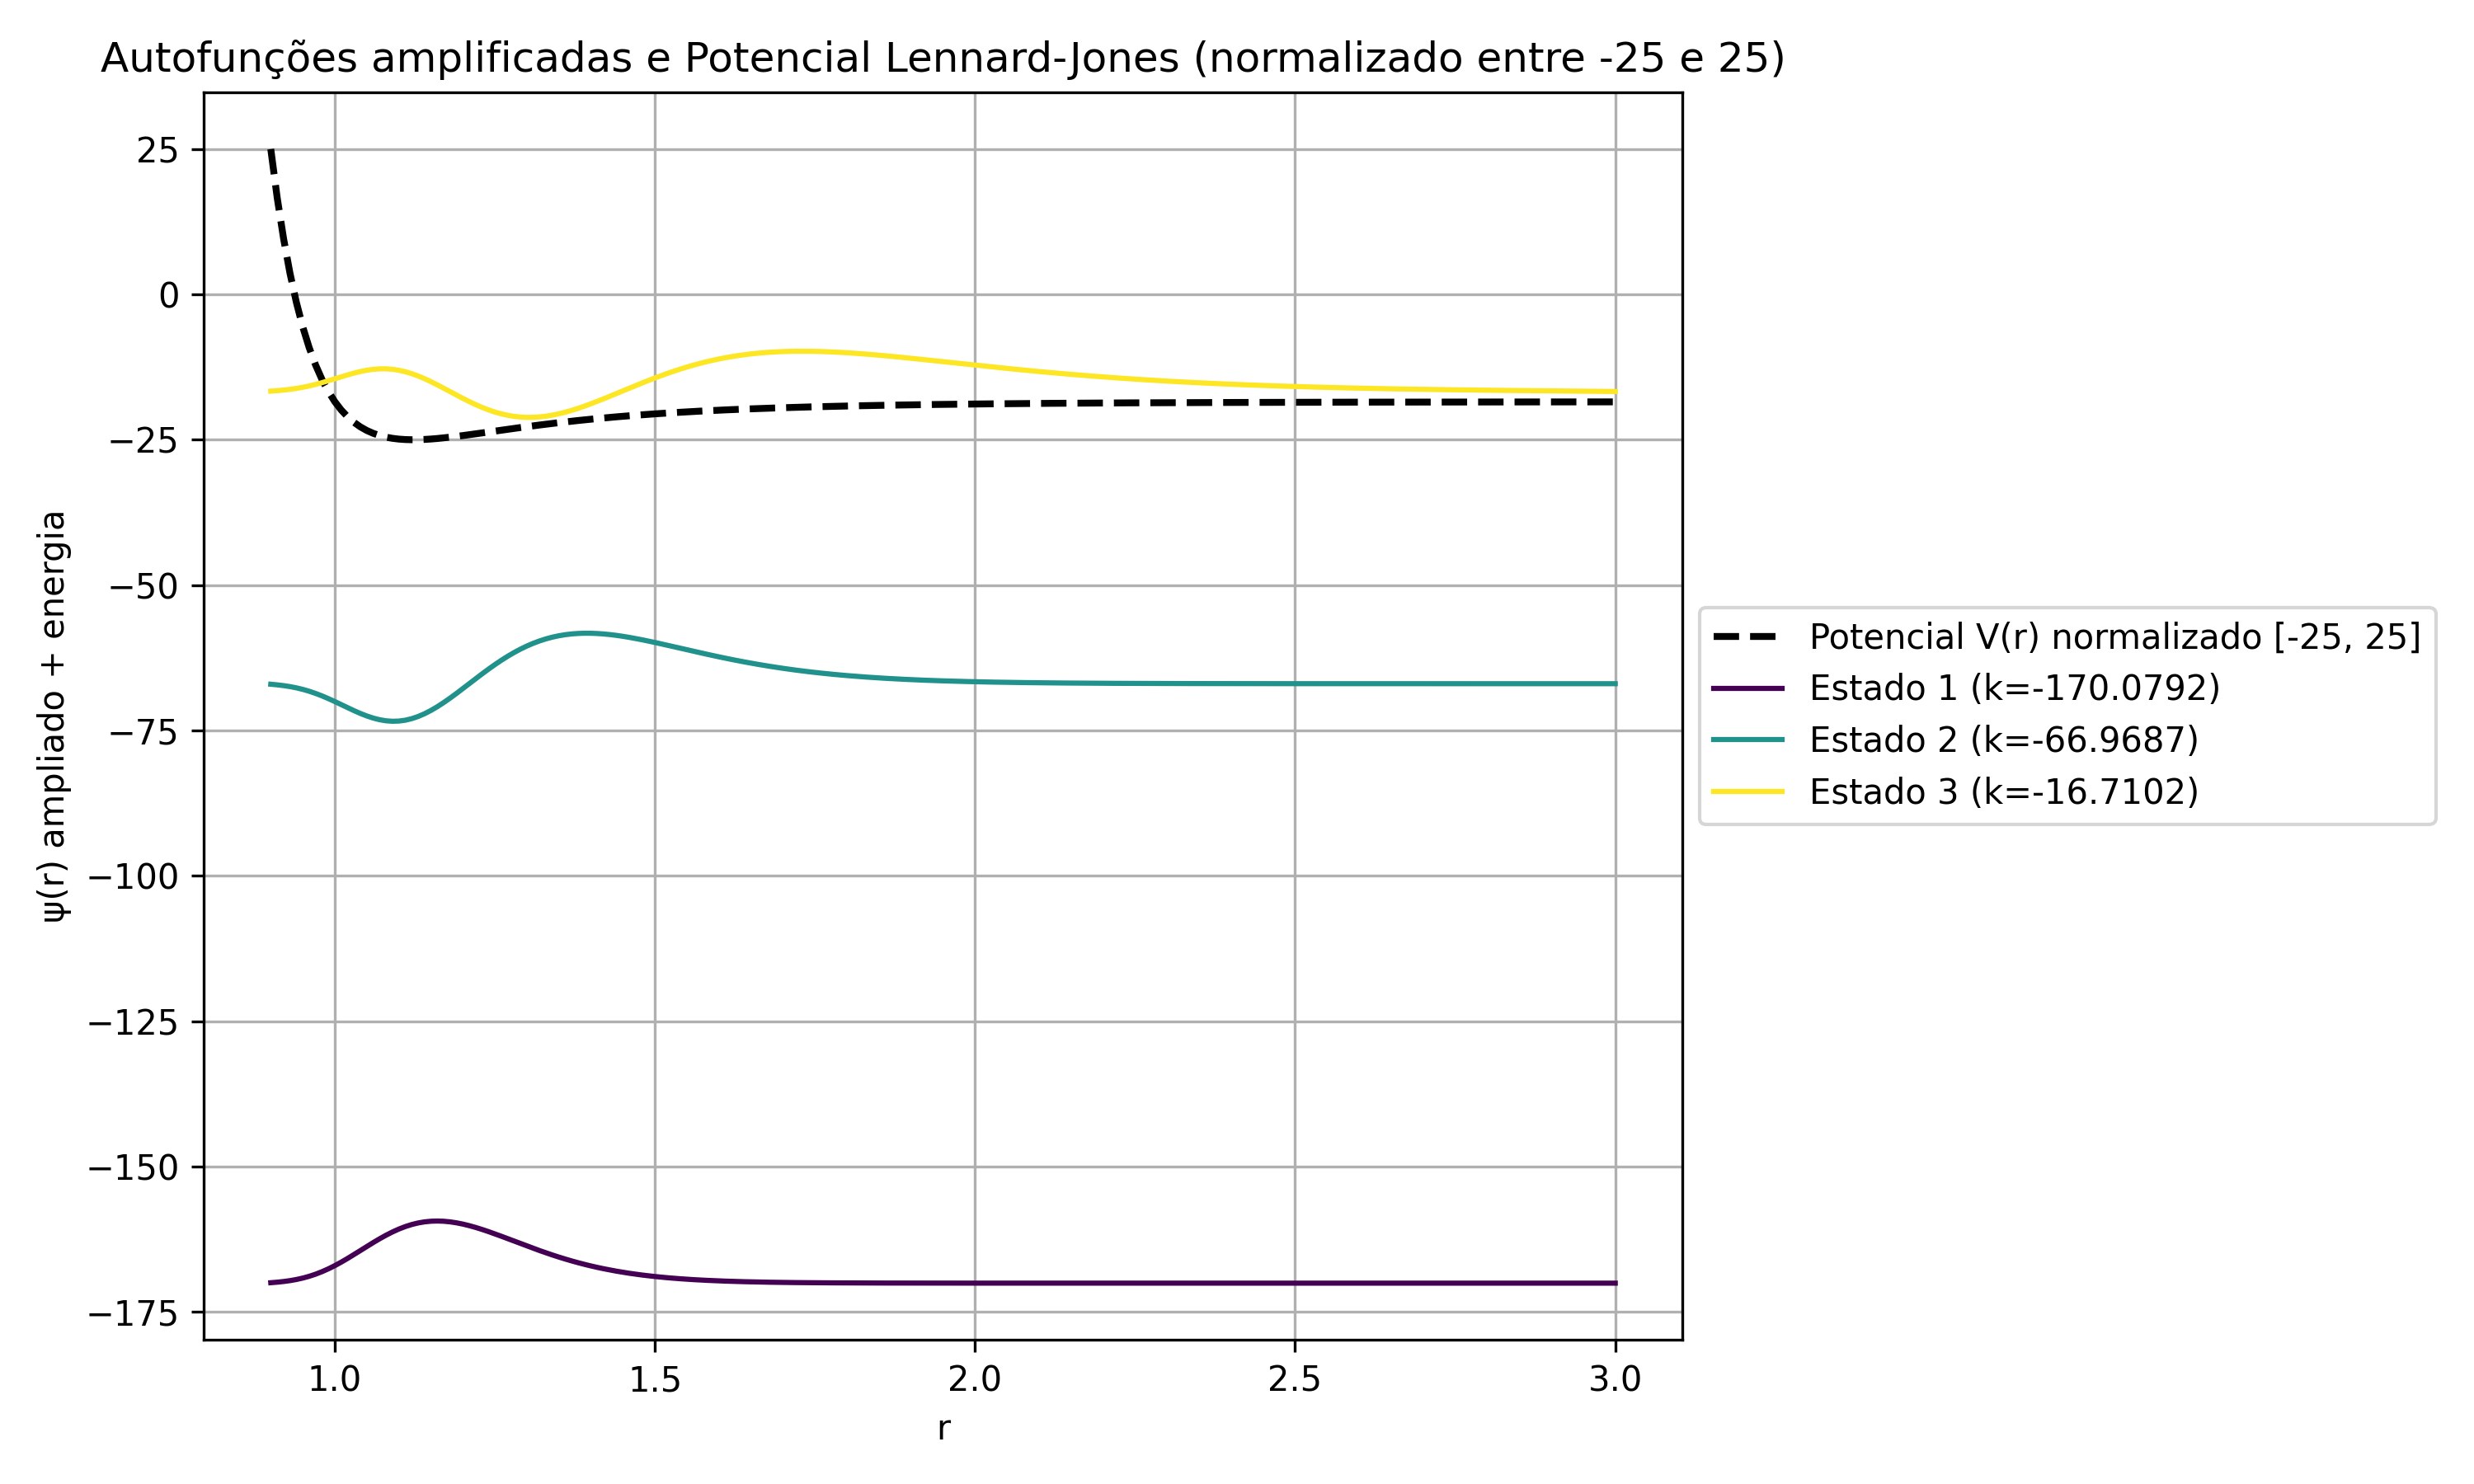
\includegraphics[scale=0.7]{../images/ex3-results-1000.png}
                \caption{Resultados para k' = 1000}
            \end{figure}

            Percebe-se que as autofun\c{c}\~oes tem car\'ater senoidal no vale do potencial e ap\'os "sa\'irem" do vale decaem exponencialmente.
            Comparam os gr\'aficos com diferentes k', percebe-se que quando maior o valor de k', menor \'e amplitude das autofun\c{c}\~oes.

        \subsection{Exerc\'icio 4}

            Tarefa: Compare a varia\c{c}\~ao de energia entre os autovalores com a varia\c{c}\~ao obtida no caso do oscilador harm\^onico.

            Faz-ze a expansão em taylor do potencial ao redor do ponto crítico:
            \begin{equation}
                V(x) = V(x_0) + V'(x_0)(x - x_0) + \frac{1}{2} V''(x_0)(x - x_0)^2
            \end{equation}
            Substituindo o potencial de Lennard-Jones obtemos:
            


\end{document}